\documentclass[lettersize,journal, one-column]{IEEEtran}
%\documentclass[journal, a4paper, onecolumn, draftcls]{IEEEtran}
\usepackage{amsmath,amsfonts}
\usepackage{algorithmic}
\usepackage{algorithm}
\usepackage{array}
\usepackage{subcaption}
\captionsetup{compatibility=false}
\usepackage{textcomp}
\usepackage{stfloats}
\usepackage{url}
\usepackage{verbatim}
\usepackage{graphicx}
\usepackage{cite}
\usepackage{varwidth}
\usepackage{hhline}
\usepackage{multirow}
\usepackage[inline]{enumitem}

\begin{document}

\title{Lightpath Length and Launch Power Estimation with Machine Learning}

\author{Shayan Hajipour}


\maketitle

\begin{abstract}
The lightpath distance between transmitter and constellation profile observation points and launch power are predicted with linear regression and support vector machine.
\end{abstract}

\section{Introduction}
\label{section:introduction}
Digital twins (DTs) with proper abstractions could be used for deriving insights, diagnosis, planning, and carrying out drills on complex systems.
An analytical DT called GNPy is already developed for signal propagation in optical networks~\cite{gnpy}.
However, sometimes analytical DTs are hard to develope.
Machine learning (ML) approach is the algorithmically simple candidate for building DTs with minimal knowledge of the subject matter.

An ML-based DT could be used to estimate lightpath (LP) attributes (e.g., launch power and distance) given In-Phase and Quadrature (IQ) optical constellation diagrams.
For example, LP launch power estimation could be used to diagnose potential discrepancies between planned, telemetry, and actual launch power estimated by DT. 
Such attribute estimations could be performed at the pass-through observation points via optical spectrum analyzers to give a better resolution of the LP status as well as the receiver site~\cite{9761942}.
After discrepancy detection, the adopted remediation measures could be initiated.

In this report, we estimate launch power and the distance between transmitter and observation point of lucid lightpaths.

\section{Dataset}
\label{section:dataset}
Two datasets are gathered for lightpath attributes estimation.
The datasets are collected by numerical simulations of two scenario configurations:
\begin{enumerate}
    \item \textit{Single link scenario}, where LPs travel up to 25 spans deployed between a transmitter and receiver.
    The observation point is the receiver, where the IQ constellation profiles consisting of 2048 symbol samples are measured as datapoints.
    The number of spans and the length of the first span are the labeled variables of the dataset.
    The length of the first span could be 80 km, 60 km, or 40 km, which are called \textit{optimal}, \textit{sub-optimal}, and \textit{degradation} modes, respectively.
    The length of other spans is 80 km.
    All simulation modes are combined and a dataset with the total number of 2250 datapoints of IQ constellation profiles is created. 
    Each datapoint consists of 2048$\times$2+1+1 columns that represent in-phase and quadrature components of symbol samples, the distance between the transmitter and the observation point, and datapoint mode.
    \item \textit{multiple links scenario}, where LPs travel 5 reconfigurable optical add-drop multiplexers (ROADMs) and 4 equal links.
    The number and length of spans in each link, launch power, and the observation point location are the labeled variables of the dataset.
    The observation point location candidates are either ingress or egress ports of ROADMs, where the IQ constellation profile consisting of 8192 symbol samples are measured as datapoints.
    A total number of 800 scans (datapoints) of IQ constellation profiles are collected.
    Each datapoint consists of 8192$\times$2+1+1+1 columns that represent in-phase and quadrature components of symbol samples, the distance between the transmitter and the observation point, the ROADM side of the observation point, and the launch power.
    The ROADM side could be either ingress or egress, which is represented by a binary number.
    The launch power is either 1 or 2 dBm, which is also represented by a binary number.
\end{enumerate}
The data generation simulation configurations are further elaborated in~\cite{data146_2022}.

\section{Machine Learning Models}
\label{section:ml_models}
We estimate the distance between the transmitter and the observation point in the single link scenario.
We also classify the launch power in the multiple links scenario since it is the lightpath configuration attribute and could be vulnerable to potential misconfiguration.
The ML pipeline for distance regression and launch power classification is shown in Fig.~\ref{figure:models}.
\begin{figure}
	\centering
    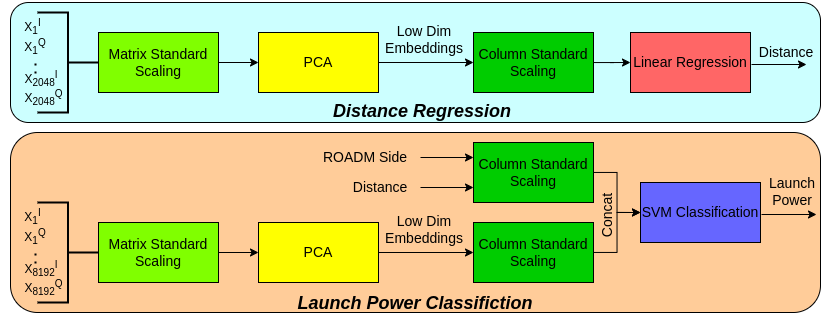
\includegraphics[width=\columnwidth]{figures/models.png}
    \caption{Lightpath attribute estimation pipelines}
	\label{figure:models}
\end{figure}
The IQ constellation profile is compressed with the principal component analysis (PCA) method.
PCA projects the original data to low dimension directions that maximize the variance.
Before PCA, the data is scaled by a custom standard scaler that operates with $\frac{(\textbf{D}-\mu)}{\sigma}$ formula, where $\textbf{D}$, $\mu$, and $\sigma$ are the IQ constellation profile, mean, and standard deviation of $\textbf{D}$ elements.
A linear regression model estimates the distance for the single link scenario after another standard scaling across columns of low dimensional embeddings resulted from PCA.
The column standard scaler operates with $\frac{\textbf{D - M}}{\mathbf{\Sigma}}$ formula, where $\textbf{D}$, $\textbf{M}$, and $\mathbf{\Sigma}$ are the IQ constellation profile, mean vector, and standard deviation vector of each column of $\textbf{D}$.
For launch power classification, the ROADM side and distance data are concatenated with the PCA embeddings after standard scaling across columns.
Then, a support vector machine (SVM) classification model classifies the launch power as depicted in Fig.~\ref{figure:models}.

\section{Results}
\label{section:results}
The proposed pipelines in Fig.~\ref{figure:models} are implemented with Python and available in~\cite{code}.
PCA models compress IQ constellation profiles to the embeddings with size 50 for either pipeline.
The datasets are split into train-test subsets with 67\%-33\% ratio.
Modules in Fig.~\ref{figure:models} are trained with the training data subset.
The testing data subset is used for validating the pipelines' performance reported in the following.
\subsection{Single Link Scenario}
\label{section:results_single_link}
The single link scenario dataset is used for distance estimation.
First, the whole dataset is compressed to embeddings of 2 dimensions with PCA.
The embeddings are decpicted in Fig.~\ref{figure:single_whole}.
It seems there is a clear distinction between the 3 modes in the 2D embeddings.
Yet, the distance-related embeddings variation is concentrated in small areas in Fig.~\ref{figure:single_optimal}.
\begin{figure}
	\centering
    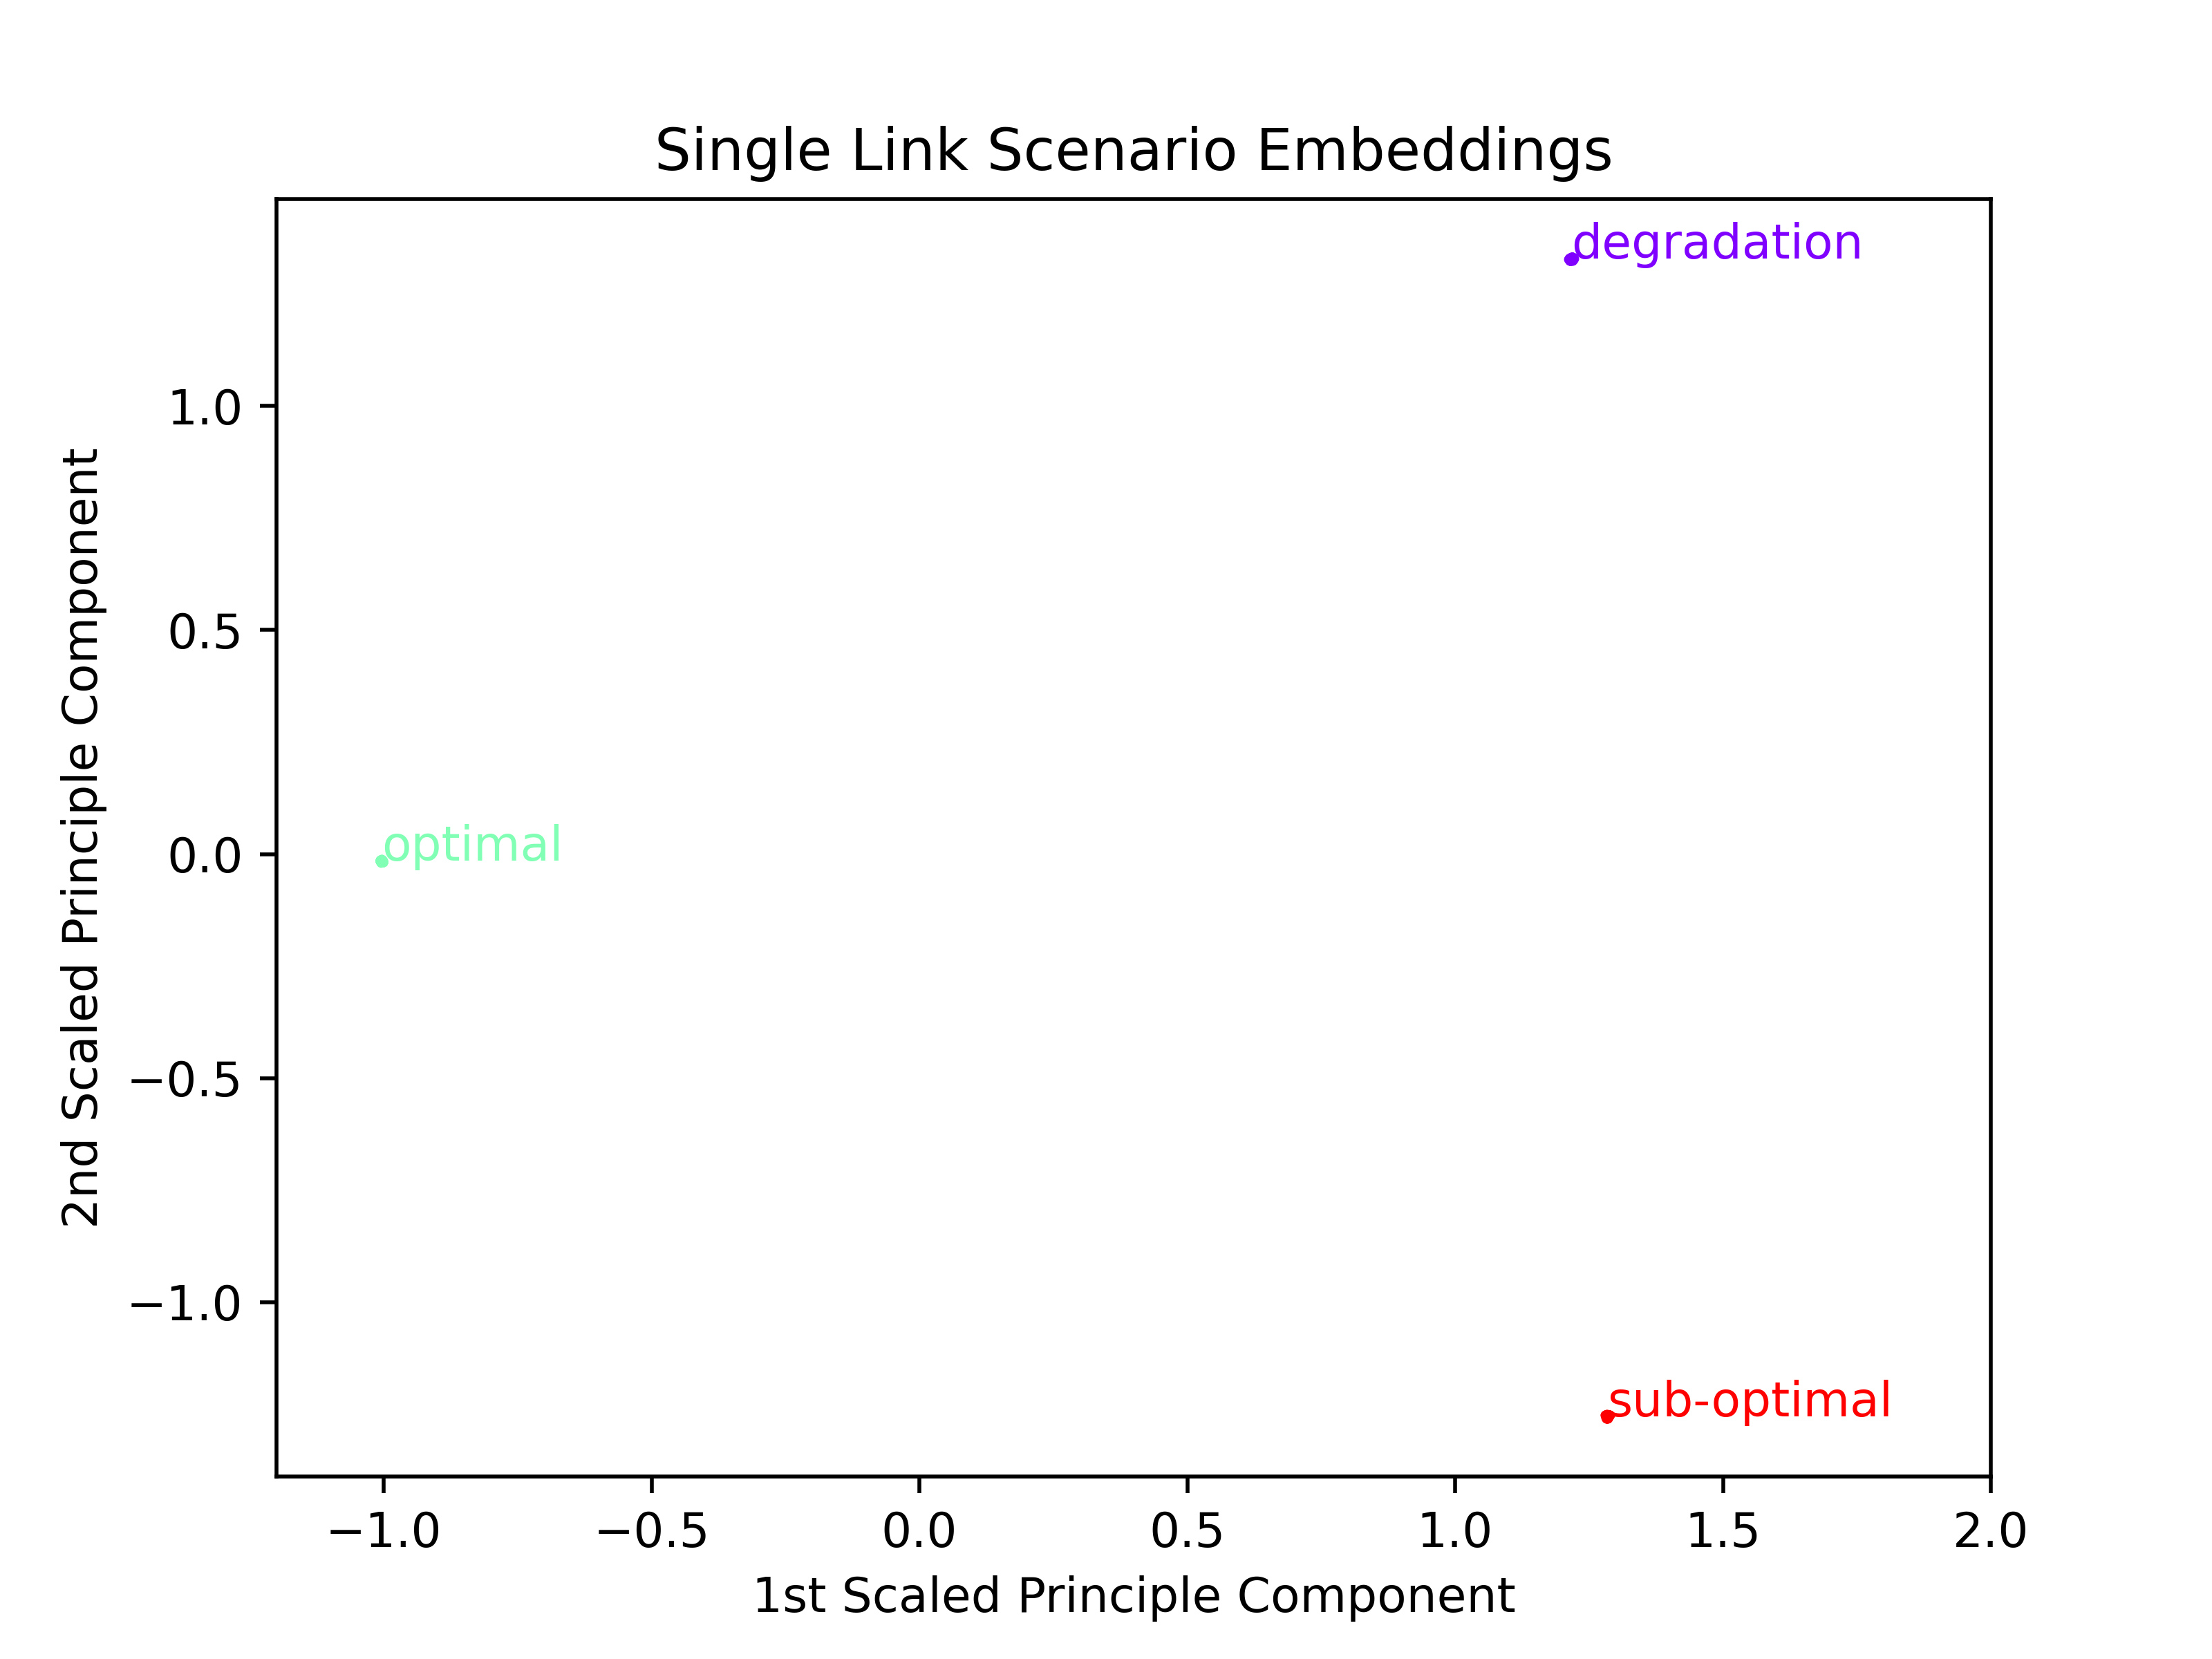
\includegraphics[width=\columnwidth]{figures/single_scenario.png}
    \caption{Single link scenario embeddings}
	\label{figure:single_whole}
\end{figure}
The same compression process is applied to datapoints of \textit{optimal} mode, which is shown in Fig.~\ref{figure:single_optimal} along with the distance between the transmitter and the observation point.
The locations of distance numbers on Fig.~\ref{figure:single_optimal} are the centeriods of distance clusters.
\begin{figure}
	\centering
    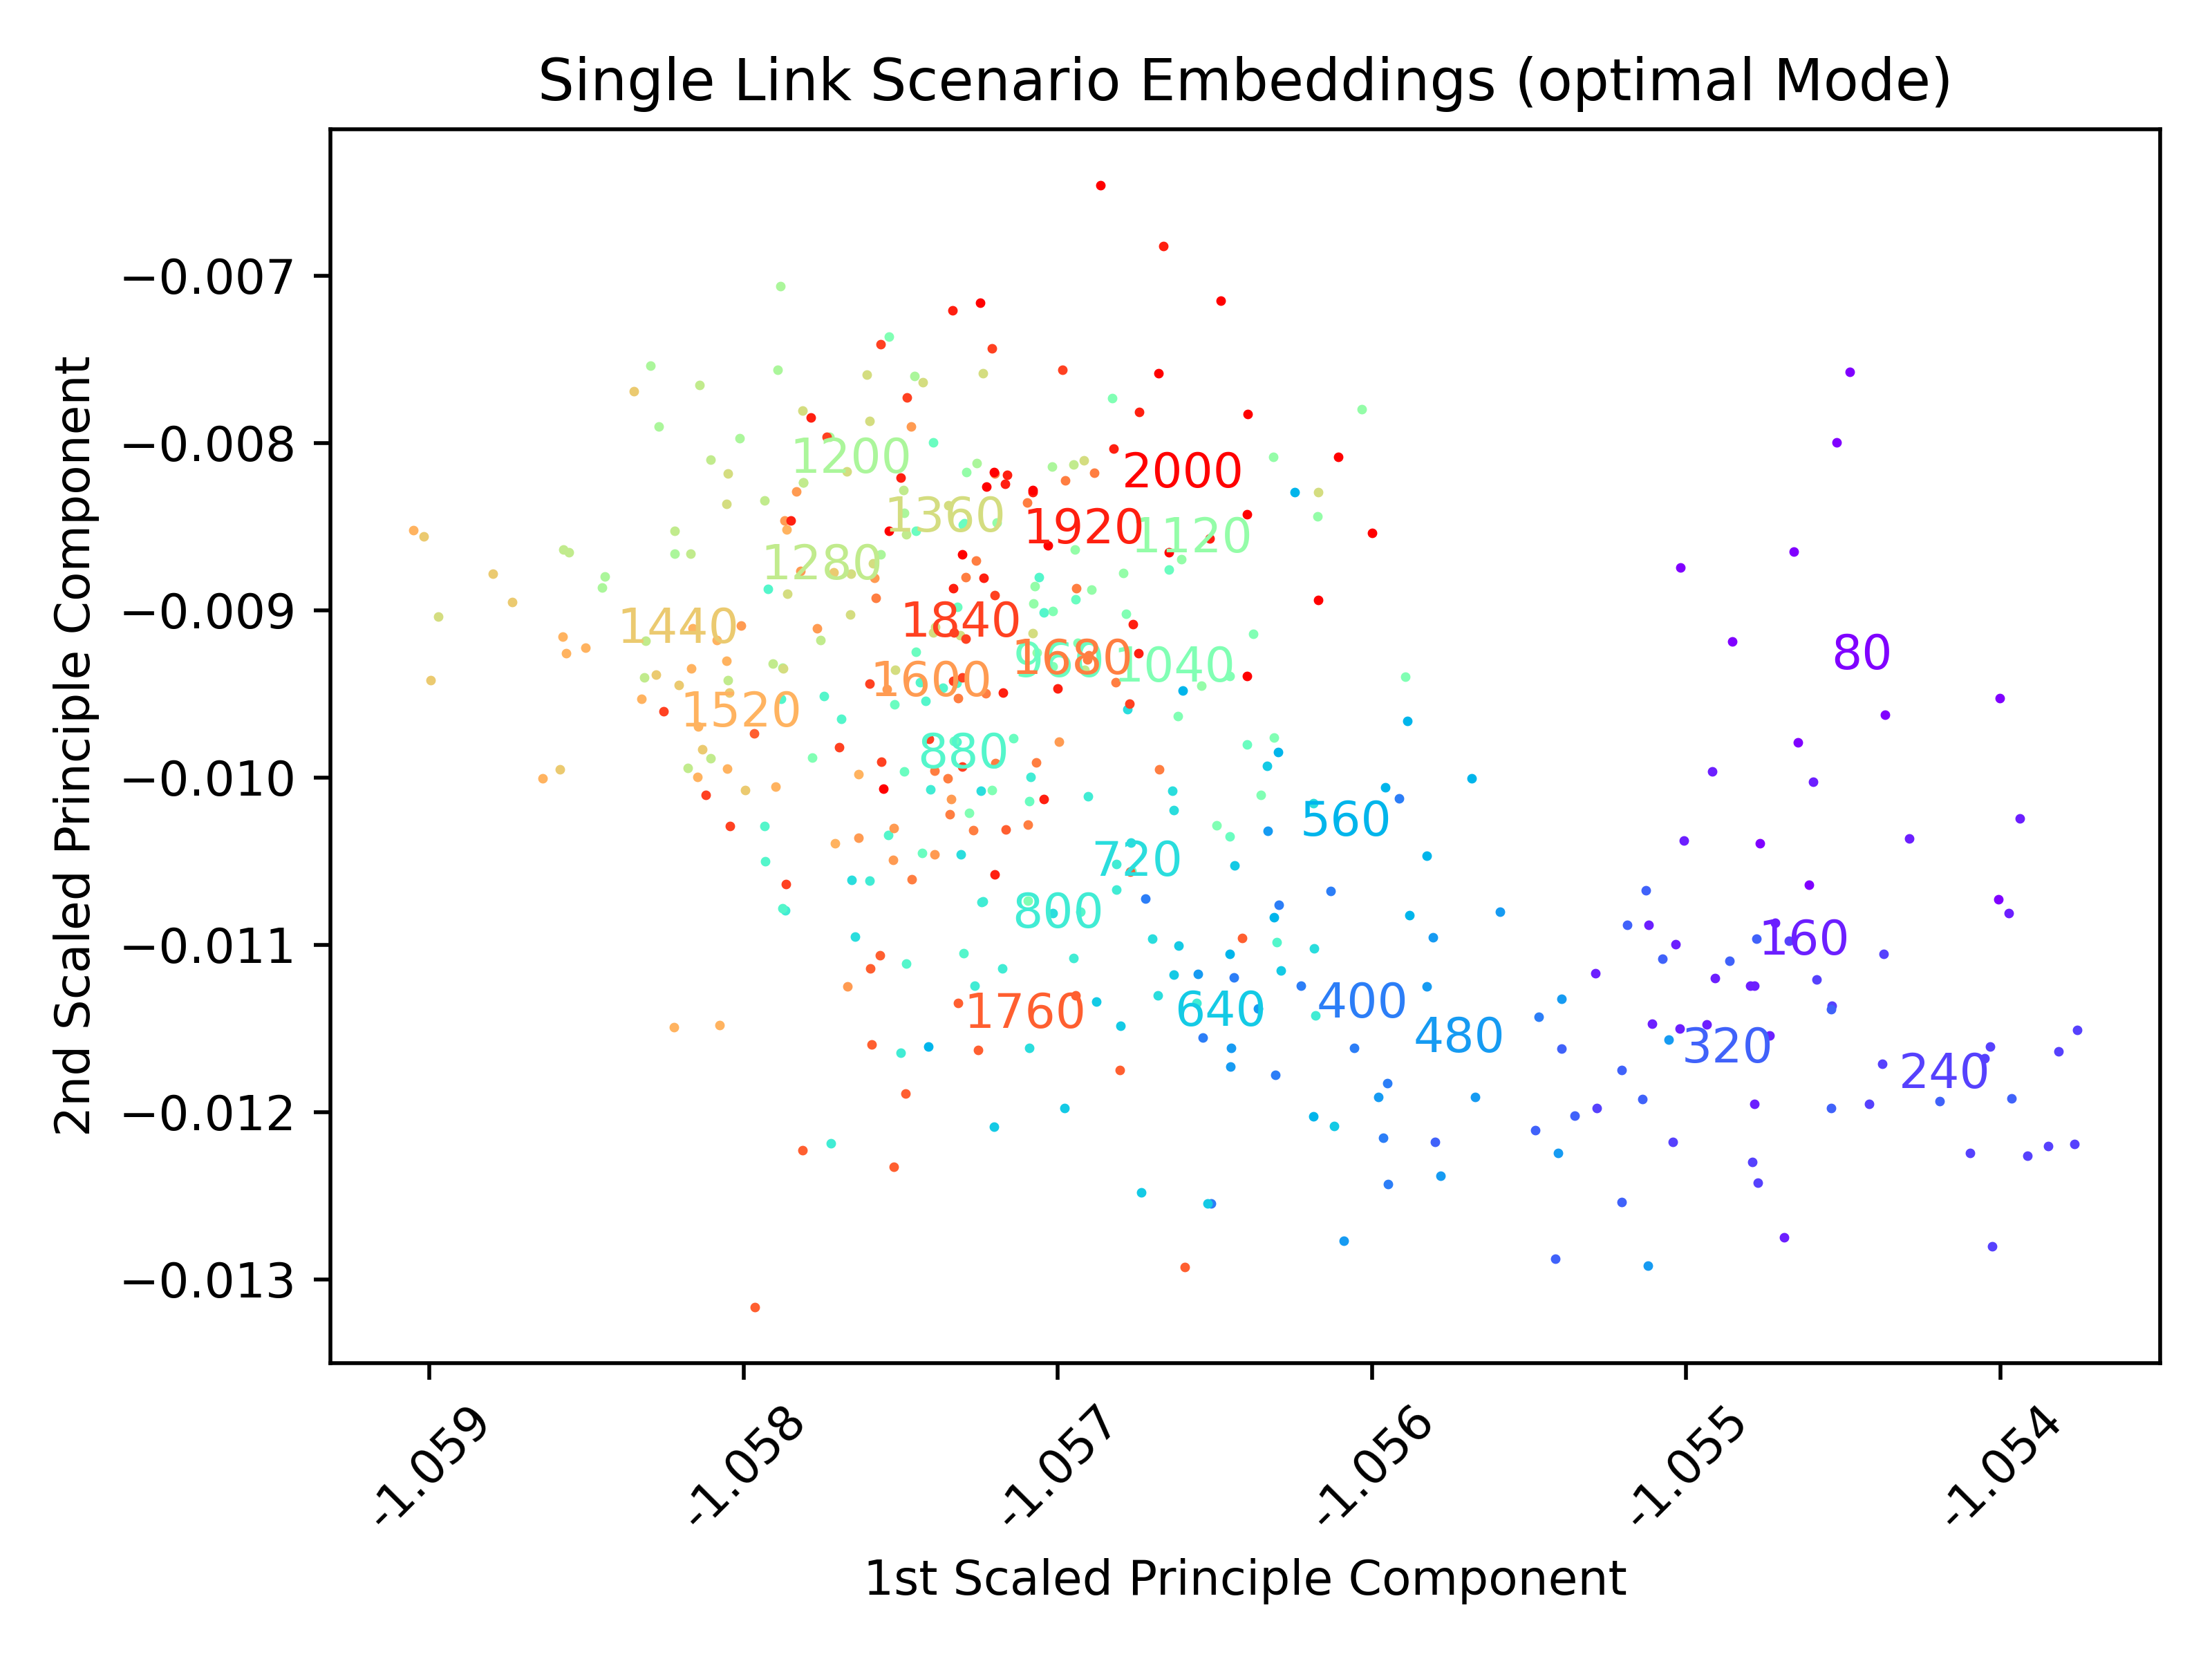
\includegraphics[width=\columnwidth]{figures/single_scenario(optimal).png}
    \caption{Single link scenario embeddings for the \textit{optimal} mode}
	\label{figure:single_optimal}
\end{figure}
The distance is distinguishable with the 2D embeddings.

We train the lightpath distance regression pipeline in Fig.~\ref{figure:models}.
The compression metrics of testing data subset after PCA is reported in Table.~\ref{table:compression}.
\begin{table}
    \centering
    \caption{Compression Metrics}
    \begin{tabular}{l l l l}
        \hline
        \hline
        Scenario & Compression Rate & MAE & MAPE \\
		\hline \\
        Single Link & 98.78\% & 0.0475 & 3.5\% \\
        Multiple Links & 99.69\% & 1.1959 & 67.22\% \\
        \hline
    \end{tabular}
    \label{table:compression}
\end{table}

The coefficient of determination (R\textsuperscript{2})-score of distance estimation with linear regression is 0.99916 for the testing data subset.

\subsection{Multiple Links Scenario}
The multiple links scenario dataset is used for launch power classification.
We compress the IQ constellation profile with PCA and depict the 2D embeddings in Fig.~\ref{figure:multiple_whole}.
\begin{figure}
	\centering
    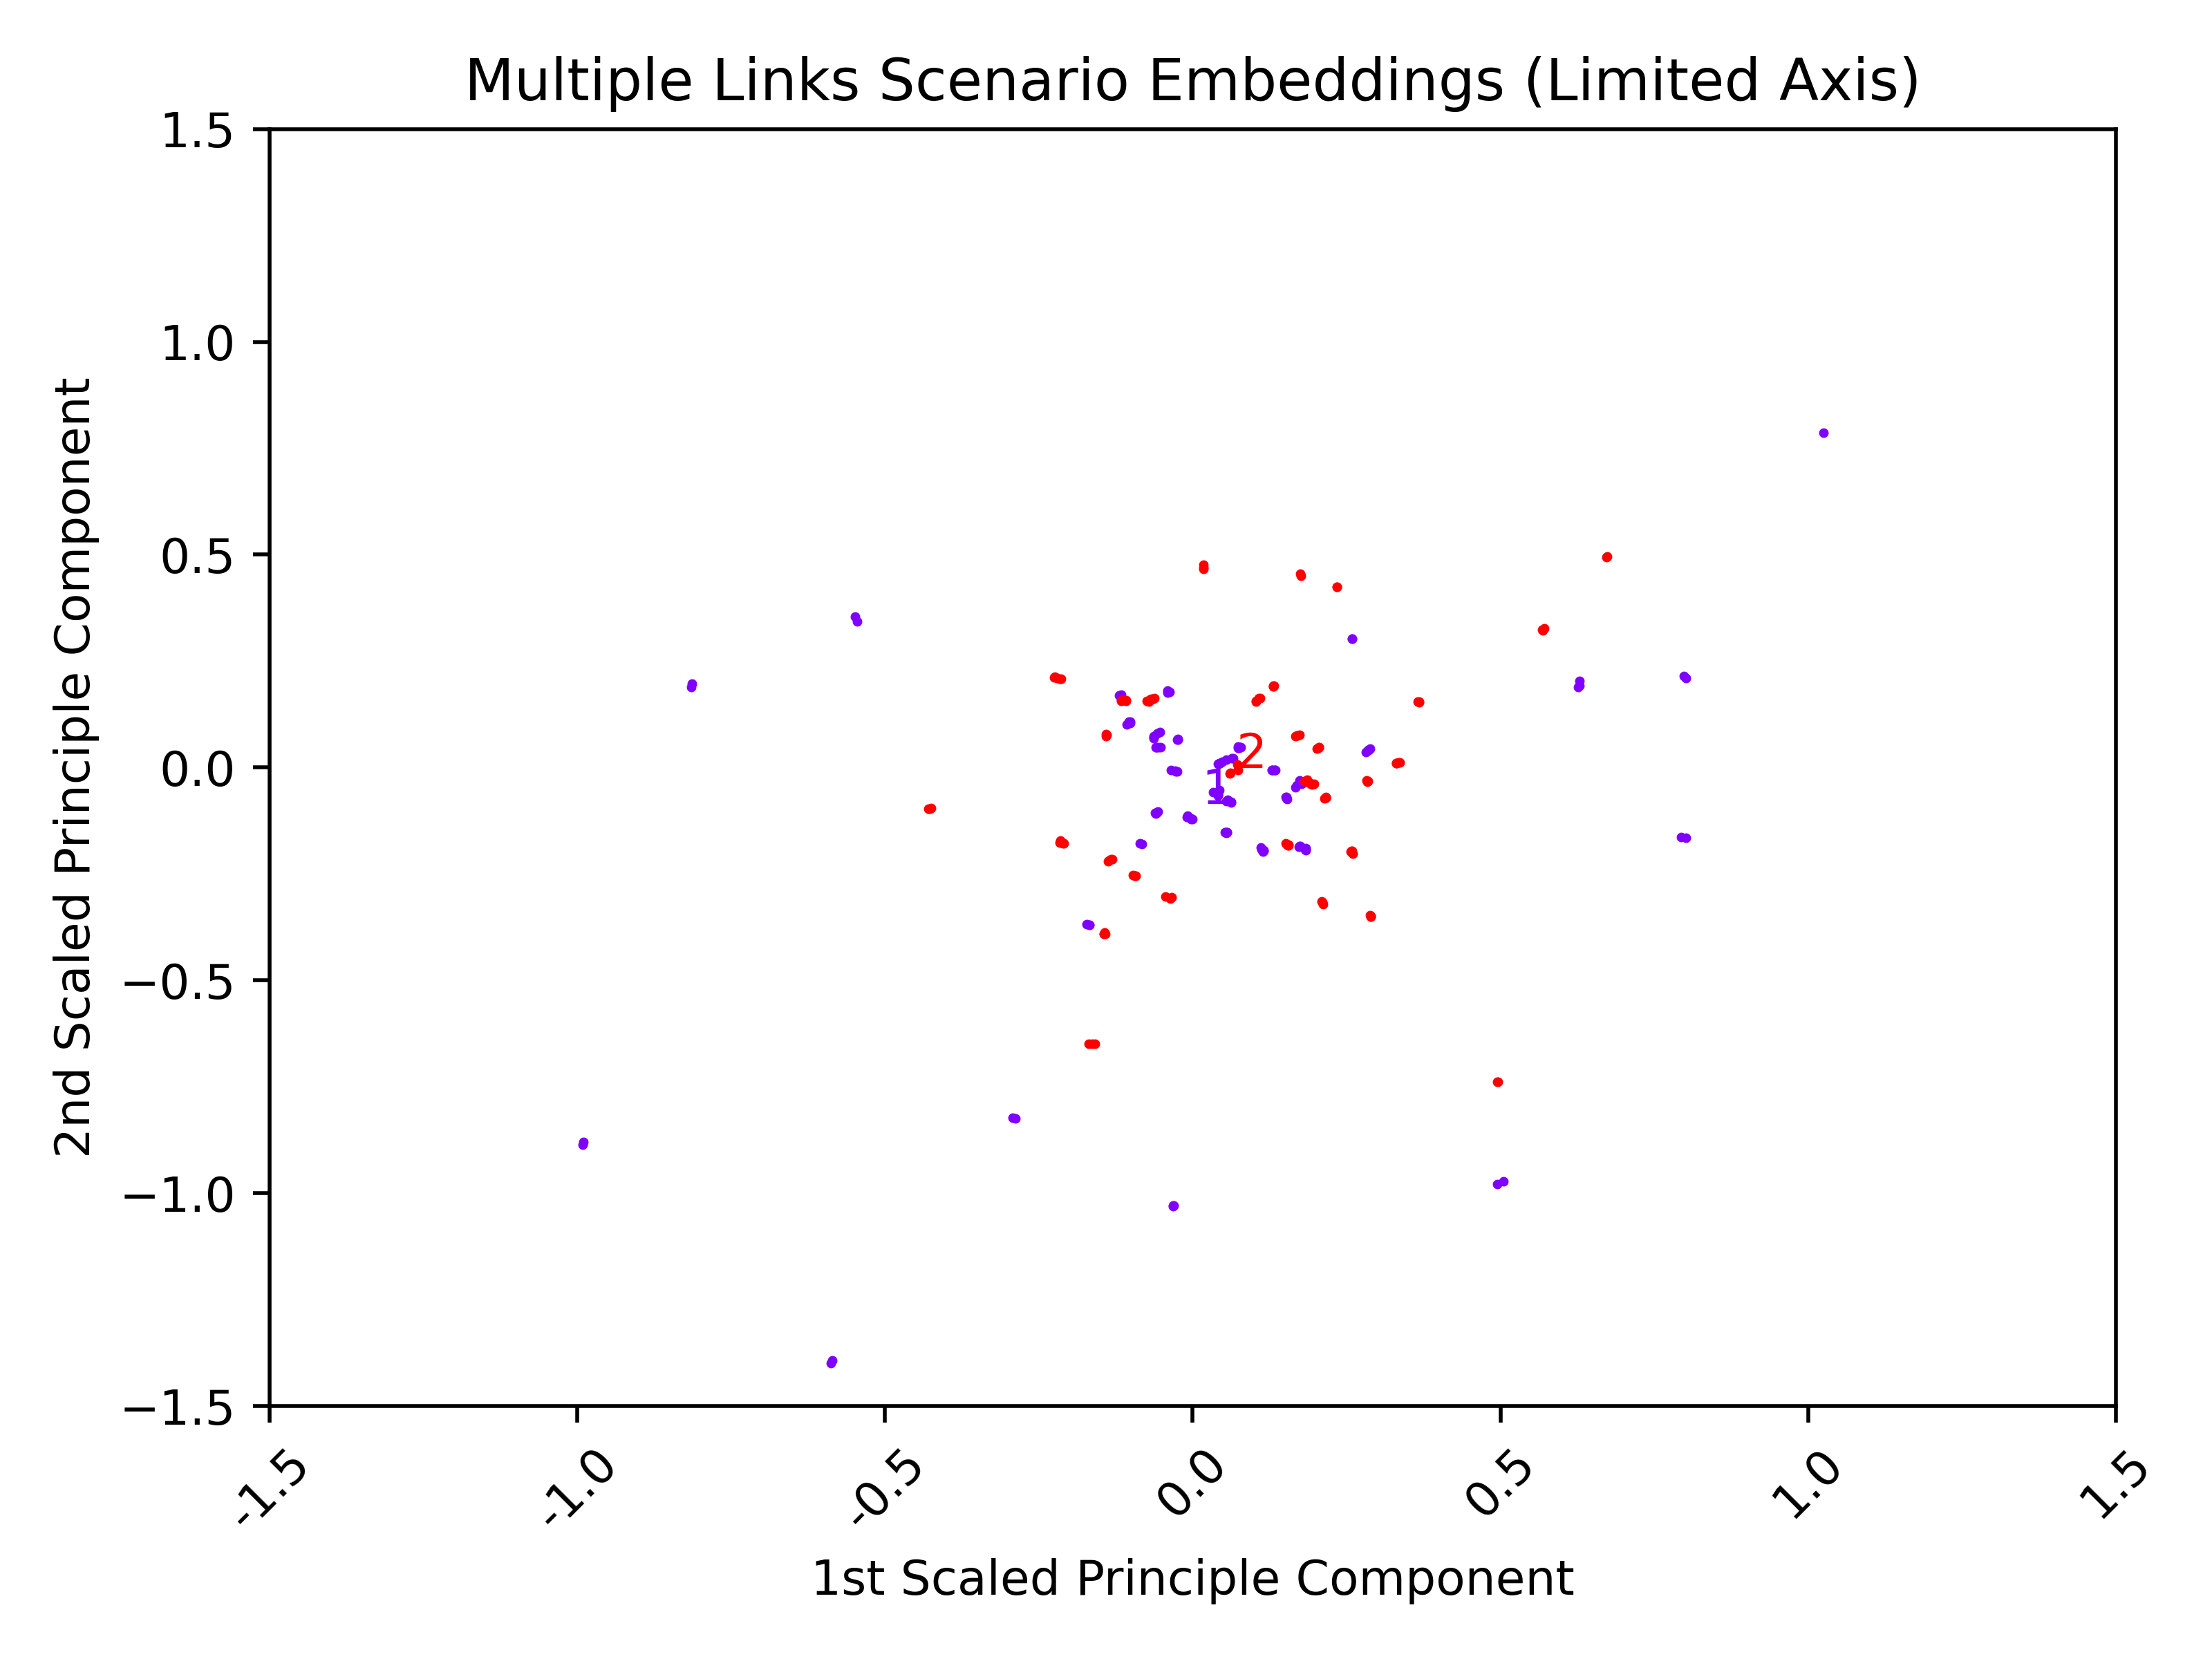
\includegraphics[width=\columnwidth]{figures/multiple_scenario_zoommed.png}
    \caption{Multiple links scenario embeddings. The 1 and 2 dBm launch power datapoint embeddings are shown with purple and red colors, respectively. Several outlier embeddings reside outside the plot scope for better visualization.}
	\label{figure:multiple_whole}
\end{figure}
There is no clear distinction between the 2D embeddings of 1 and 2 dBm constellation profiles.
However, increasing the size of embeddings might create clusters associated with launch power.

We train the launch power classification pipeline in Fig.~\ref{figure:models}.
The confusion matrix of the testing data subset is reported in Table.~\ref{table:confusion_mat}.
\begin{table}
    \centering
    \caption{Launch Power Classification Confusion Matrix}
    \begin{tabular}{l l l}
        & 1 dBm (Prediction) & 2 dBm (Prediction) \\
        \cline{2-3}
        1 dBm (Target) & \multicolumn{1}{|c|}{132} & \multicolumn{1}{c|}{0} \\
        \cline{2-3}
        2 dBm (Target) & \multicolumn{1}{|c|}{34} & \multicolumn{1}{c|}{98} \\
        \cline{2-3}
    \end{tabular}
    \label{table:confusion_mat}
\end{table}
The accuracy of classification is 0.87121 based on Table.~\ref{table:confusion_mat}

\section{Conclusion}
\label{section:conclusion}
The IQ constellation profile could be used to estimate lightpath attributes.
The report investigates launch power and distance between transmitter and observation point estimation use cases with ML.
The use cases do not require information about the dynamics of optical signal propagation in optical networks.
Estimations are derived with the raw dataset. 

The study could be extended in several directions, including: investigation of more efficient methods for compression (e.g., Gaussian mixture models), using more complex ML models for classification and regression, hyperparameter search for finding the best ML configurations that optimize the metrics, and error analysis of dataset cohorts.


\begin{thebibliography}{1}
\bibliographystyle{IEEEtran}

\bibitem{gnpy}TIP. GNPy: Optical Route Planning and DWDM Network Optimization. {\em GitHub Repository}. (2023), https://github.com/Telecominfraproject/oopt-gnpy

\bibitem{9761942}Ruiz, M., Sequeira, D. \& Velasco, L. Deep learning-based real-time analysis of lightpath optical constellations [Invited]. {\em Journal Of Optical Communications And Networking}. \textbf{14}, C70-C81 (2022)

\bibitem{data146_2022}Ruiz Ramírez, M., Velasco Esteban, L. \& Sequeira, D. Optical Constellation Analysis (OCATA). (CORA.Repositori de Dades de Recerca,2022), https://doi.org/10.34810/data146

\bibitem{code}Hajipour, S. Lightpath Length and Launch Power Estimation with Machine Learning. {\em GitHub Repository}. (2023), https://github.com/hprshayan/lightpath-attribute-estimation




\end{thebibliography}
\end{document}


